\section{Missing Values}    
\begin{tcolorbox}[title=Easier Said Than Done]
Obviously, the best way to treat missing data is not to have any. \\[-0.6cm]
\begin{flushright}
-- T. Orchard, M. Woodbury, \textit{A Missing Information Principle: Theory and Applications}, 1972
\end{flushright}
\end{tcolorbox}
\noindent Why does it matter that some values may be \textbf{missing}? Well, they can potentially introduce bias into the analysis, which is rarely (if at all) a good thing, but, more pragmatically, they may interfere with the functioning of most analytical methods, which can not easily accommodate missing observations without breaking down.\footnote{For instance, The canonical equation $\mathbf{X}^{\!\top}\mathbf{X}\mathbf{\beta}=\mathbf{X}^{\!\top}\mathbf{Y}$ of linear regression cannot be solved as $\mathbf{X}^{\!\top}\mathbf{X}$ is not defined if some observations are missing.}  \par Consequently, when faced with missing observations, analysts have two options: they can either \textbf{discard} the missing observation (which is not typically recommended, unless the data is missing completely randomly), or they can \textbf{create a replacement value} for the missing observation (the \textbf{imputation} strategy has drawbacks since we can never be certain that the replacement value is the true value, but is often the best available option; information in this section is taken partly from \cite{DP_Shinnie,DP_RLVHS,DP_vB,DP_R}).
\newpage\noindent  Blank fields come in 4 flavours: \begin{itemize}[noitemsep]\item \textbf{nonresponse} -- an observation was expected but none was entered; \item  \textbf{data entry issues} -- an observation was recorded but was not entered in the dataset; \item \textbf{invalid entries} -- an observation was recorded but was considered invalid and has been removed, and \item  \textbf{expected blanks} -- a field has been left blank, but not unexpectedly so.
\end{itemize}
Too many missing values of the first three types can be indicative of \textbf{issues with the data collection process}, while too many missing values of the fourth type can be indicative of \textbf{poor questionnaire design} (see \cite{DP_PDC} for a brief discussion on these topics). \newl Either way, missing values cannot simply be \textbf{ignored}: either the
\begin{itemize}[noitemsep]
\item corresponding record is removed from the dataset (not recommended without justification, as doing so may cause a loss of auxiliary information and may bias the analysis results), or 
\item missing value must be \textbf{imputed} (that is to say,  a reasonable replacement value must be found).
\end{itemize}
\subsection{Missing Value Mechanisms} The relevance of an imputation method is dependent on the underlying \textbf{missing value mechanism}; values may be 
\begin{itemize}[noitemsep]
\item \textbf{missing completely at random} (MCAR) -- the item absence is independent of its value or of the unit's auxiliary variables (e.g., an electrical surge randomly deletes an observation in the dataset); 
\item \textbf{missing at random} (MAR) -- the item absence is not completely random, and could, in theory, be accounted by the unit's complete auxiliary information, if available (e.g., if women are less likely to tell you their age than men for societal reasons, but not because of the age values themselves), and 
\item \textbf{not missing at random} (NMAR) -- the reason for nonresponse is related to the item value itself (e.g., if illicit drug users are less likely to admit to drug use than teetotalers).
\end{itemize}
The consultant's main challenge in that regard is that the missing mechanism cannot typically be determined with any degree of certainty.
\subsection{Imputation Methods}
There are numerous statistical \textbf{imputation} methods. They each have their strengths and weaknesses; consequently, consultants and analysts should take care to select a method which is appropriate for the situation at hand.\footnote{Imputation methods work best under MCAR or MAR, but keep in mind that they all tend to produce \textbf{biased estimates}.}
\begin{figure*}[t]
\centering
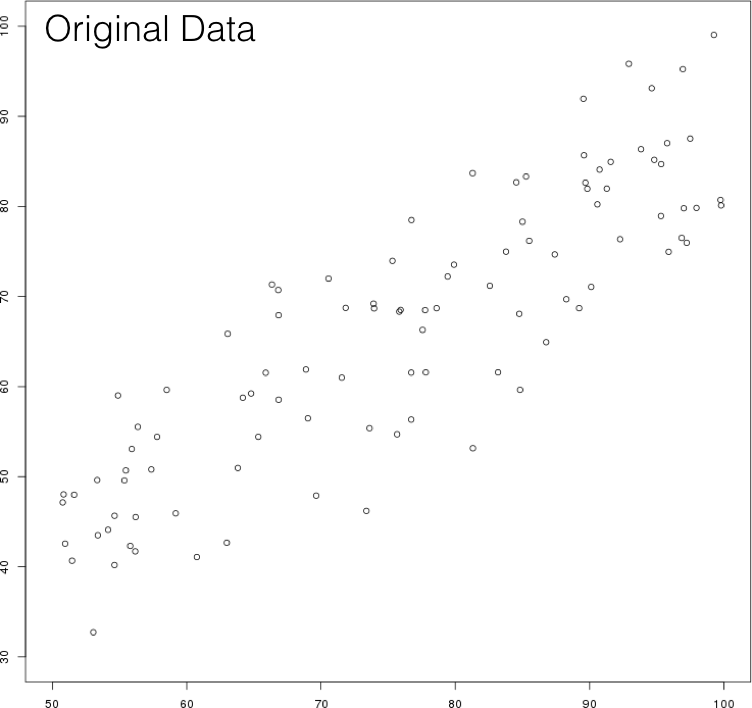
\includegraphics[width=0.5\textwidth]{Images/original.png}
\caption[\small Dr.\@ Vanderwhede's original \textit{Advanced Retroencabulation} dataset]{\small Dr.\@ Vanderwhede's original \textit{Advanced Retroencabulation} dataset; mid-term grades ($x-$axis), final exam grades ($y-$axis).} \label{fig:ori}\hrule
\end{figure*}
\begin{itemize}[noitemsep]
\item In \textbf{list-wise deletion}, all units with at least one missing value are removed from the dataset. This straightforward imputation strategy assumes MCAR, but it can introduce bias if MCAR does not hold, and it leads to a reduction in the sample size and an increase in standard errors.
\item In \textbf{mean} or \textbf{most frequent imputation}, the missing values are substituted by the average or most frequent value in the unit's subpopulation group (stratum). This commonly-used approach also assumes MCAR, but it can creates distortions in the underlying distributions (such as a spike at the mean) and create spurious relationships among variables.
\item  In \textbf{regression} or \textbf{correlation imputation}, the missing values are substituted using a regression on the other variables. This model assumes MAR and trains the regression on units with complete information, in order to take full advantage of the auxiliary information when it is available. However, it artificially reduces data variability and produces over-estimates of correlations.
\item In \textbf{stochastic regression imputation}, the regression estimates are augmented with random error terms added. Just as in regression estimation, the model assumes MAR; an added benefit is that it tends to produce estimates that ``look'' more realistic than regression imputation, but it comes with an increased risk of type I error (false positives) due to small standard errors.
\item\textbf{Last observation carried forward} (LOCF) and its cousin \textbf{next observation carried backward} (NOCB) are useful for longitudinal data; a missing value can simply be substituted by the previous or next value. LOCF and NOCB can be used when the values do not vary greatly from one observation to the next, and when values are MCAR. Their main drawback is that they may be too ``generous'' for studies that are trying to determine the effect of a treatment over time, say. 
\item Finally, in \textbf{$k$-nearest-neighbour imputation}, a missing entry in a MAR scenario is substituted by the average (or median, or mode) value from the subgroup of the $k$ most similar complete respondents. This requires a notion of \textbf{similarity} between units (which is not always easy to define reasonably). The choice of $k$ is somewhat arbitrary and can affect the imputation, potentially distorting the data structure when it is too  large. 
\end{itemize}
\begin{center}
    \rule{0.5\linewidth}{.4pt}
\end{center}
\begin{figure*}[t]
\centering
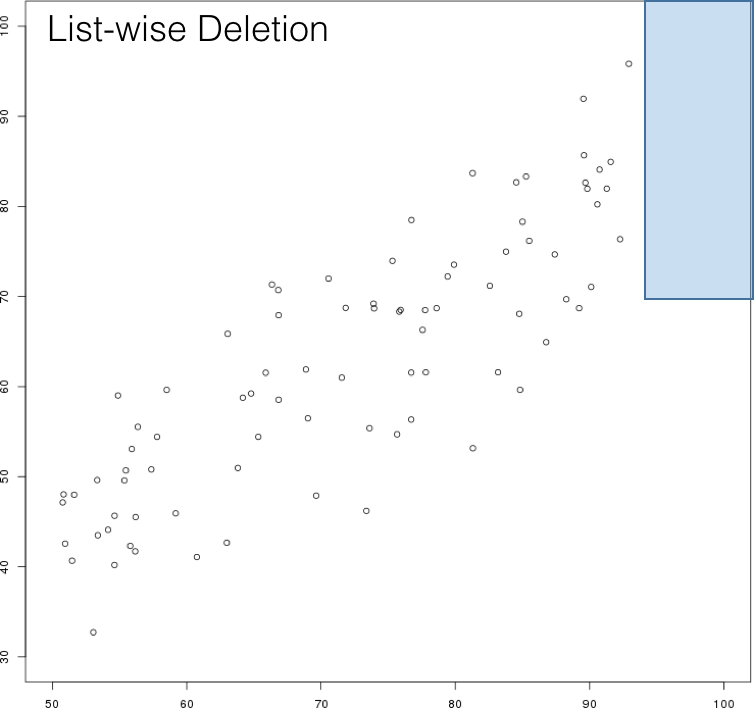
\includegraphics[width=0.48\textwidth]{Images/listwisedeletion.png}
\quad
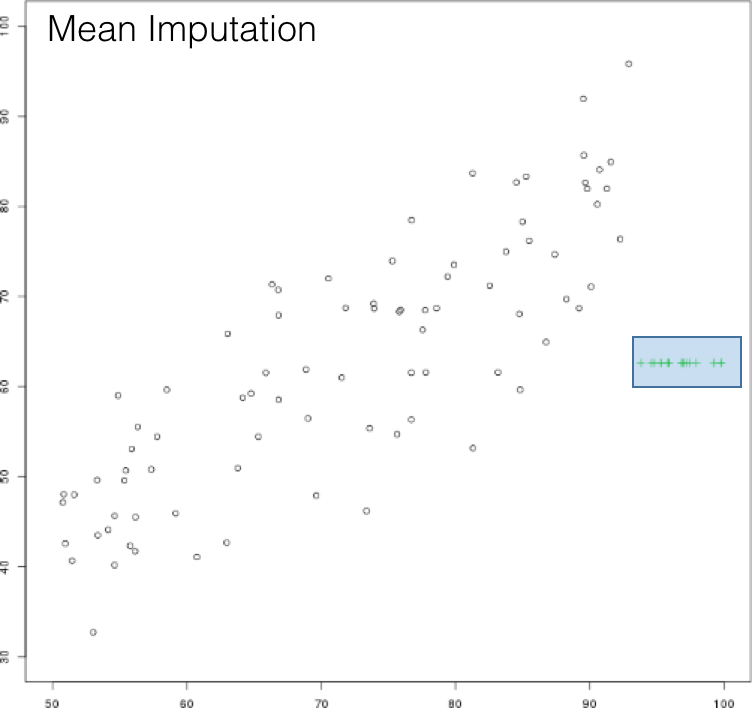
\includegraphics[width=0.48\textwidth]{Images/mean.png} \\
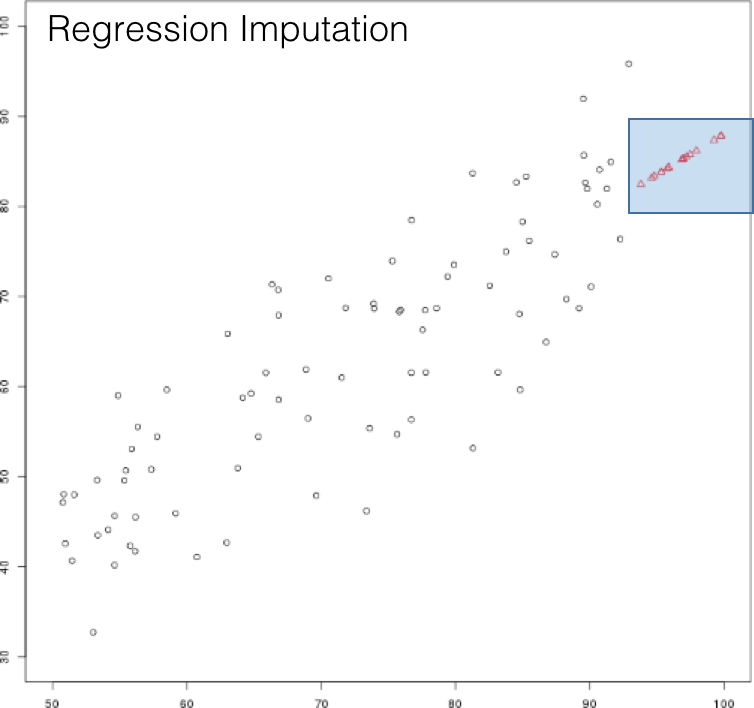
\includegraphics[width=0.48\textwidth]{Images/regression.png} 
\quad
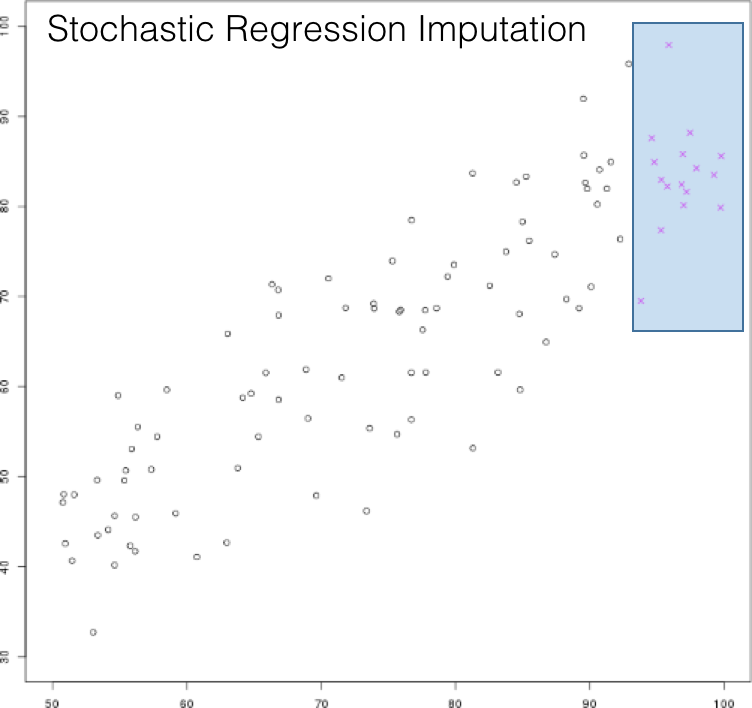
\includegraphics[width=0.48\textwidth]{Images/stochastic.png}
\caption[\small Imputed values for Dr.\@ Vanderwhede's dataset]{\small Imputed values for Dr.\@ Vanderwhede's dataset.}
\label{fig:theimputations}\hrule
\end{figure*}
What does imputation look like in practice? \newl Consider the following scenario (which is, somewhat embarrassingly, based on a true story): after marking the final exams of the 100 students who did not drop her course in \textit{Advanced Retroencabulation} at State University, Dr.\@ Helga Vanderwhede plots the final exam grades ($y$) against the mid-term exam grades ($x$) as in Figure~\ref{fig:ori}. \par She takes a quick look at the data and sees that final exam grades are \textbf{correlated} with mid-term exam grades: students who perform well on the mid-term tend to perform well on the final, and students who perform poorly on the mid-term tend to perform poorly on the final, as is usually the case. \par She also sees that there is a fair amount of variability in the data: the noise is not very tight around the (eye-balled) line of best fit. \par Furthermore, she realizes that the final exam was harder than the students expected\footnote{The slope of the line of best fit is smaller than $1$.} -- she suspects that they simply did not prepare for the exam seriously (and not that she made the exam too difficult, no matter what her ratings on \texttt{RateMyProfessor.com} suggest), as most of them could not match their mid-term exam performance. 
\newl As Dr.\@ Vanderwhede comes to term with her disappointment, she takes a deeper look at the numbers, at some point sorting the dataset according to the mid-term exam grades. It looks like good old Mary Sue performed better on the final than on the mid-term (where her performance was already superlative), scoring the only perfect score.\newpage\noindent  What a great student Mary Sue is! And such a fantastic person -- in spite of her superior intellect, she is adored by all of her classmates, thanks to her sunny disposition and willingness to help at all times. If only all students were like Mary Sue... \par She continues to toy with the spreadsheet until the phone rings. After a long and exhausting conversation with Dean Bitterman about teaching loads and State University's reputation, Dr.\@ Vanderwhede returns to the spreadsheet and notices in horror that she has accidentally deleted the final exam grades of all students with a mid-term grade greater than 92. \newl What is she to do? \newl A technically-savvy consultant would advise her to either undo her changes or to close the file without saving the changes,\footnote{Or to re-enter the final grades by comparing with the physical papers} but let's assume for the time being that, in full panic mode, the only solution that comes to her mind is to impute the missing values. \par She knows that the missing final grades are MAR (and not MCAR since she remembers sorting the data along the $x$ values); she produces the imputations shown in Figure~\ref{fig:theimputations}. She remembers what the data looked like originally, and concludes that the best imputation method is the stochastic regression model.
\newl
But this only applies to this specific example. In general, that might not be the case, however, due to various \textit{No Free Lunch} results.\footnote{``There ain't no such thing as a free lunch'' -- there is no guarantee that a method that works best for a dataset even works well for another.} \newpage \noindent The principal take-away from this example is that various imputation strategies lead to different outcomes, and perhaps more importantly, that even though the imputed data might ``look'' like the true data, we have no way to measure its \textbf{departure from reality} -- any single imputed value is likely to be completely off. \par Mathematically, this might not be problematic, as the average departure is likely to be relatively small, but in a business or personal context, this might create gigantic problems  -- how is Mary Sue likely to feel about Dr.\@ Vanderwhede's solution in the previous example? How is Dean Bitterman likely to react, if he finds out about the imputation scenario from irrate students? \newl Even though such questions are not quantitative in nature, their answer will impact any actionable  solution.  
\subsection{Multiple Imputation}
Another drawback of imputation is that it tends to increase the noise in the data, because the imputed data is treated as the \textit{actual} data. \par  In \textbf{multiple imputation}, the impact of that noise can be reduced by consolidating the analysis outcome from multiple imputed datasets. Once an imputation strategy has been selected on the basis of the (assumed) missing value mechanism, 
\begin{enumerate}[noitemsep]
\item the imputation process is repeated $m$ times to produce $m$ versions of the dataset;
\item each of these datasets is analyzed, yielding $m$ outcomes, and  
\item the $m$ outcomes are pooled into a single result for which the mean, variance, and confidence intervals are known.
\end{enumerate}\newpage\noindent 
On the plus side, multiple imputation is \textbf{easy to implement}, \textbf{flexible}, as it can  be used in a most situations (MCAR, MAR, even NMAR in certain cases), and it accounts for \textbf{uncertainty} in the imputed values. \par However, $m$ may need to be quite \textbf{large} when the values are missing in large quantities from many of the dataset's features, which can substantially slow down the analyses. \par There may also be additional technical challenges when the output of the analyses is not a single value but some more complicated object.\newl A generalization of multiple imputation was used by Transport Canada to predict the Blood Alcohol Level (BAC) content level in fatal traffic collisions that involved pedestrians \cite{CP_BAC}.

